
\section{Resultados experimentais}

\begin{frame}{Metodologia}{Representações de fórmulas}
	\begin{figure}
		\centering
		
		\raisebox{3.5\height}{$(p \leftrightarrow p) \leftrightarrow (p \leftrightarrow p)$}
		\hspace{.5cm}
		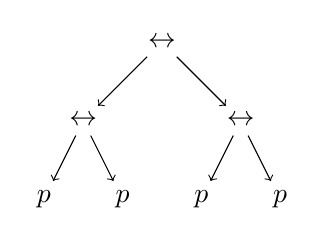
\begin{tikzpicture}
		\tikzset{vertex/.style = {}}
		\tikzset{edge/.style = {->}}
		
		\node[vertex]  (1) at (   0,    1) {$\leftrightarrow$};
		\node[vertex]  (2) at (  -1,    0) {$\leftrightarrow$};
		\node[vertex]  (3) at (   1,    0) {$\leftrightarrow$};
		\node[vertex]  (4) at (-1.5,   -1) {$p$};
		\node[vertex]  (5) at (-0.5,   -1) {$p$};
		\node[vertex]  (6) at ( 0.5,   -1) {$p$};
		\node[vertex]  (7) at ( 1.5,   -1) {$p$};
		
		\draw[edge] (1) to  (2);
		\draw[edge] (1) to  (3);
		\draw[edge] (2) to  (4);
		\draw[edge] (2) to  (5);
		\draw[edge] (3) to  (6);
		\draw[edge] (3) to  (7);
		\end{tikzpicture}
		\hspace{1cm}
		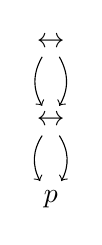
\begin{tikzpicture}
		\tikzset{vertex/.style = {}}
		\tikzset{edge/.style = {->}}
		
		\node[vertex]  (1) at (   0,    1) {$\leftrightarrow$};
		\node[vertex]  (2) at (   0,    0) {$\leftrightarrow$};
		\node[vertex]  (3) at (   0,   -1) {$p$};
		
		\draw[edge] (1) to [bend right] (2);
		\draw[edge] (1) to [bend left ] (2);
		\draw[edge] (2) to [bend right] (3);
		\draw[edge] (2) to [bend left ] (3);
		\end{tikzpicture}
		
		\hspace{1.2cm}\pause Cadeia\hspace{2.3cm}\pause Árvore sintática\hspace{1.8cm}\pause DAG
	\end{figure}
\end{frame}

\begin{frame}{Metodologia}{Implementação}
	Foi implementado um programa em C++ 11 que realiza, em ordem, as seguintes transformações:
	\begin{enumerate}
		\pause\item Análise sintática \pause (de cadeia para árvore)
		\pause\item Conversão para FNN \pause (simplifica \pause e permite testar a conjectura)
		\pause\item Aplainamento \pause ($p \vee (q \vee r) \longmapsto p \vee q \vee r$\pause, mais simplificações)
		\pause\item Conversão para DAG \pause (de árvore para DAG)
		\pause\item Renomeamento \pause (Boy de la Tour e proposto)
		\pause\item Conversão para FNC \pause (opcional: simplificações)
		\pause\item Conversão de DAG para cadeia
	\end{enumerate}
\end{frame}

\begin{frame}{Metodologia}{Implementação -- Renomeamento}
	No algoritmo de Boy de la Tour, quando $\psi = \psi_1 \vee ... \vee \psi_n$:
	
	\pause $$a_{\psi_i}^\phi = a_\psi^\phi \cdot \prod_{j \neq i} p(\psi_j)$$
	
	\pause Ao processar cada $\psi_i$, temos as seguintes alternativas:
	\begin{enumerate}
		\pause\item Calcular $a_{\psi_i}^\phi$ com um laço.
		\pause\item Calcular $a_\psi^\phi \cdot \prod_{j} p(\psi_j)$ antes e dividir por $p(\psi_i)$.
		\pause\item Calcular uma tabela de sufixos antes e combinar com um prefixo atualizado após cada iteração. \pause Fazemos assim!
	\end{enumerate}
\end{frame}

\begin{frame}{Metodologia}{Implementação -- Renomeamento}
	Além disso, pode ocorrer:
	
	\pause
	\begin{figure}
		\centering
		
		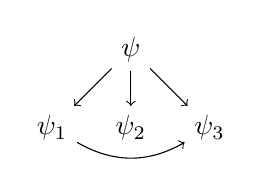
\begin{tikzpicture}
		\tikzset{vertex/.style = {}}
		\tikzset{edge/.style = {->}}
		
		\node[vertex]  (1) at (   0,    1) {$\psi$};
		\node[vertex]  (2) at (  -1,    0) {$\psi_1$};
		\node[vertex]  (3) at (   0,    0) {$\psi_2$};
		\node[vertex]  (4) at (   1,    0) {$\psi_3$};
		
		\draw[edge] (1) to  (2);
		\draw[edge] (1) to  (3);
		\draw[edge] (1) to  (4);
		\draw[edge] (2) to [bend right] (4);
		\end{tikzpicture}
	\end{figure}
	
	\pause Portanto, é necessária uma ordenação topológica:
	
	\pause
	\begin{figure}
		\centering
		
		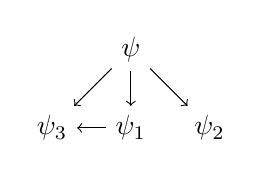
\begin{tikzpicture}
		\tikzset{vertex/.style = {}}
		\tikzset{edge/.style = {->}}
		
		\node[vertex]  (1) at (   0,    1) {$\psi$};
		\node[vertex]  (2) at (  -1,    0) {$\psi_3$};
		\node[vertex]  (3) at (   0,    0) {$\psi_1$};
		\node[vertex]  (4) at (   1,    0) {$\psi_2$};
		
		\draw[edge] (1) to  (2);
		\draw[edge] (1) to  (3);
		\draw[edge] (1) to  (4);
		\draw[edge] (3) to  (2);
		\end{tikzpicture}
	\end{figure}
\end{frame}

\begin{frame}{Metodologia}{Experimentos propostos}
	Sobre um \textit{benchmark} tradicional de 1200 fórmulas, foram executadas as seguintes combinações:
	
	\pause
	\vspace{.5cm}
	\begin{tabular}{l|cccccccccc}
		Combinação         & 1 & 2 & 3 & 4 & 5 & 6 & 7 & 8 & 9 & 10 \\ \hline
		Análise sintática  & X & X & X & X & X & X & X & X & X & X  \\
		Conversão para FNN & X & X & X & X & X & X & X & X & X & X  \\
		Aplainamento       & X & X & X & X & X & X & X & X & X & X  \\
		Conversão para DAG &   &   &   &   &   &   & X & X & X & X  \\
		Renomeamento       &   &   & 1 & 1 & 2 & 2 & 1 & 1 & 2 & 2  \\
		Conversão para FNC & 1 & 2 & 1 & 2 & 1 & 2 & 1 & 2 & 1 & 2  \\
	\end{tabular}
	
	\vspace{.4cm}
	\pause Em seguida, executamos um decisor de VAL baseado em FNC.
\end{frame}

\begin{frame}{Resultados e análise}{Combinações sem renomeamento}
	Combinação 1: sem renomeamento, sem simplificação\\
	Combinação 2: sem renomeamento, com simplificação
	
	\begin{itemize}
		\pause\item Na Combinação 1, 73\% excedeu limite de memória.
		\pause\item Na Combinação 2, 67\% excedeu limite de memória e 1\% excedeu limite de tempo.
		\pause\item Nos 27\% em que a transformação terminou em C1 e C2, somente 5 fórmulas (menos de 1\% do \textit{benchmark}) mantiveram o tamanho em C2.
	\end{itemize}
	
	\pause Simplificação é bom. \pause Mas não é suficiente!
\end{frame}

\begin{frame}{Resultados e análise}{Testando a conjectura para árvores lineares}
	Combinação 3: árvore, Boy de la Tour, sem simplificação\\
	Combinação 5: árvore, algoritmo proposto, sem simplificação
	
	\pause A transformação terminou em C3 e C5 para 49\% das fórmulas.
	
	\pause Nestes 49\%, Boy de la Tour e o algoritmo proposto produziram o mesmo número de cláusulas.
\end{frame}

\begin{frame}{Resultados e análise}{Comparações entre árvores e DAGs}
	Combinações $3,4,5,6$: árvore\\
	Combinações $7,8,9,10$: DAG
	
	\vspace{.1cm}
	\pause \begin{center}Comparando número de cláusulas.\end{center}
	\begin{scriptsize}
	\begin{tabular}{l|c|c|c|c|l}
		& $C_3 \times C_7$ & $C_4 \times C_8$ & $C_5 \times C_9$ & $C_6 \times C_{10}$ \\ \hline
		$C_i$ foi melhor em & 0 (0\%)     & 5 (0\%)     & 0 (0\%)     & 6 (1\%)      & fórmulas. \\
		$C_{i+4}$ foi melhor em   & 179 (15\%)  & 177 (15\%)  & 367 (31\%)  & 358 (30\%)   & fórmulas. \\
	\end{tabular}
	\end{scriptsize}
	
	\vspace{.1cm}
	\pause Claro, DAGs simplesmente permitem renomeamento global!
\end{frame}

\begin{frame}{Resultados e análise}{Comparações entre árvores e DAGs}
	Combinações $3,4,5,6$: árvore\\
	Combinações $7,8,9,10$: DAG
	
	\vspace{-.4cm}
	\pause
	\begin{center}
		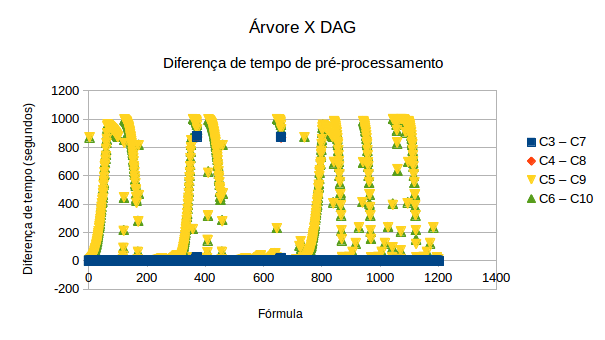
\includegraphics[scale=.5]{arvore_x_dag_time}
	\end{center}
	
	\vspace{-.6cm}
	\pause Claro, DAG é uma estrutura mais compacta!
\end{frame}

\begin{frame}{Resultados e análise}{Comparações entre árvores e DAGs}
	Combinações $3,4,5,6$: árvore\\
	Combinações $7,8,9,10$: DAG
	
	\vspace{-.4cm}
	\pause
	\begin{center}
		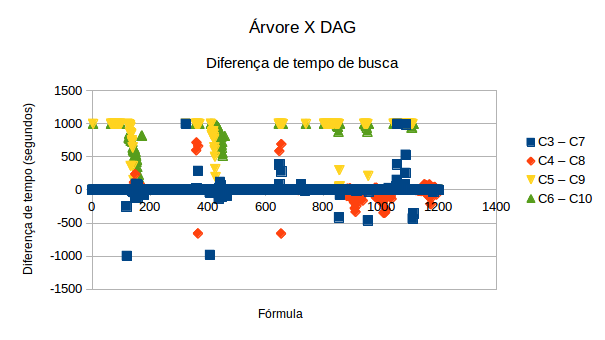
\includegraphics[scale=.5]{arvore_x_dag_ptime}
	\end{center}
	
	\vspace{-.6cm}
	\pause Primeiro indício! \pause Converter para DAG é essencial.
\end{frame}

\begin{frame}{Resultados e análise}{Comparações entre os algoritmos de renomeamento}
	Combinações $7,8$: Boy de la Tour, sem e com simplificação\\
	Combinações $9,10$: Algoritmo proposto, sem e com simplificação
	
	\pause \begin{center}Comparando número de cláusulas.\end{center}
	\begin{itemize}
		\pause\item A transformação terminou em C7 e C9 para 73\% das fórmulas.
		\pause\item Em 3\% do \textit{benchmark}, C7 produziu menos cláusulas, com $\max \{|C7-C9| \} = 3$.
		\pause\item Em 8\%, C9 produziu menos cláusulas, com $\max \{|C7-C9| \} = 1.572.786$, onde C9 produziu 78 cláusulas.
	\end{itemize}
\end{frame}

\begin{frame}{Resultados e análise}{Comparações entre os algoritmos de renomeamento}
	Combinações $7,8$: Boy de la Tour, sem e com simplificação\\
	Combinações $9,10$: Algoritmo proposto, sem e com simplificação
	
	\vspace{-.4cm}
	\pause
	\begin{center}
		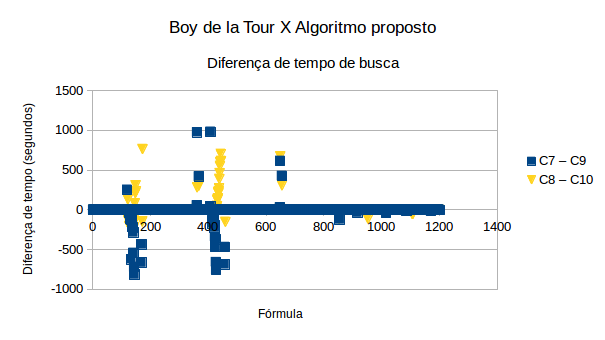
\includegraphics[scale=.5]{boy_x_knapsack_ptime}
	\end{center}
	
	\vspace{-.6cm}
	\pause Cada algoritmo leva vantagem em famílias de fórmulas específicas.
\end{frame}

\begin{frame}{Resultados e análise}{Tempo de busca em função do número de cláusulas}
	\begin{center}
		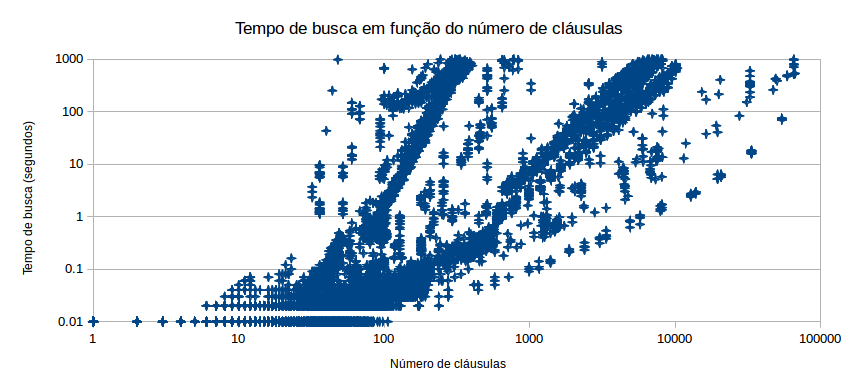
\includegraphics[scale=.45]{ptime}
	\end{center}
\end{frame}

\begin{frame}{Resultados e análise}{Tempo de busca em função do número de cláusulas}
	\begin{center}
		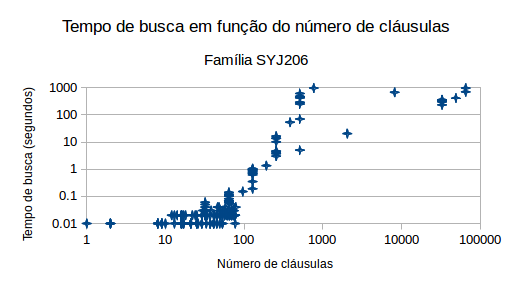
\includegraphics[scale=.6]{ptime_SYJ}
	\end{center}
	
	\pause Então, sim!
\end{frame}
